\subsection{Interaction functions}
Empirical chemical research has led to rules and concepts for MM involving atoms and their interactions with each other, e.g., bond lengths, torsional dihedral angles, or electrostatic interactions.\cite{Morse1929, Pauling1934, } 
The interaction functions represent these rules and concepts, and the required parameters can be retrieved from the system topology and coordinates. 
Usually interaction functions are split into two groups, the intra molecular $V^{bonded}$ and the inter moleculare interactions $V^{nonbonded} $. \cite{}
In the following, we will present the interaction functions used in this thesis and the GROMOS54A7 force field\cite{Schmid2011}. 

\paragraph{Bond Stretching}
Covalent bonds are an elemental part of chemistry, with the essential property of the bond-length. From the given set of coordinates r, the bond length between to covalently connected atoms can be calculated as,
\begin{equation}
    b_{ij} = \sqrt{(\vec{r}_i-\vec{r}_j)^{2}}
\end{equation}

The bond length is used to calculate the potential energy $V^{bond}$ that is in most force fields based on the harmonic oscillator, \cite{}
\begin{equation}
    V^{bond}(b_{ij}; K_{b_{ij}}, b_{ij}^0)~=~\frac{1}{2} K_{b_{ij}} (b_{ij}-b^0_{ij})^2 \\
\end{equation}.

\begin{figure}[h]
    \centering
    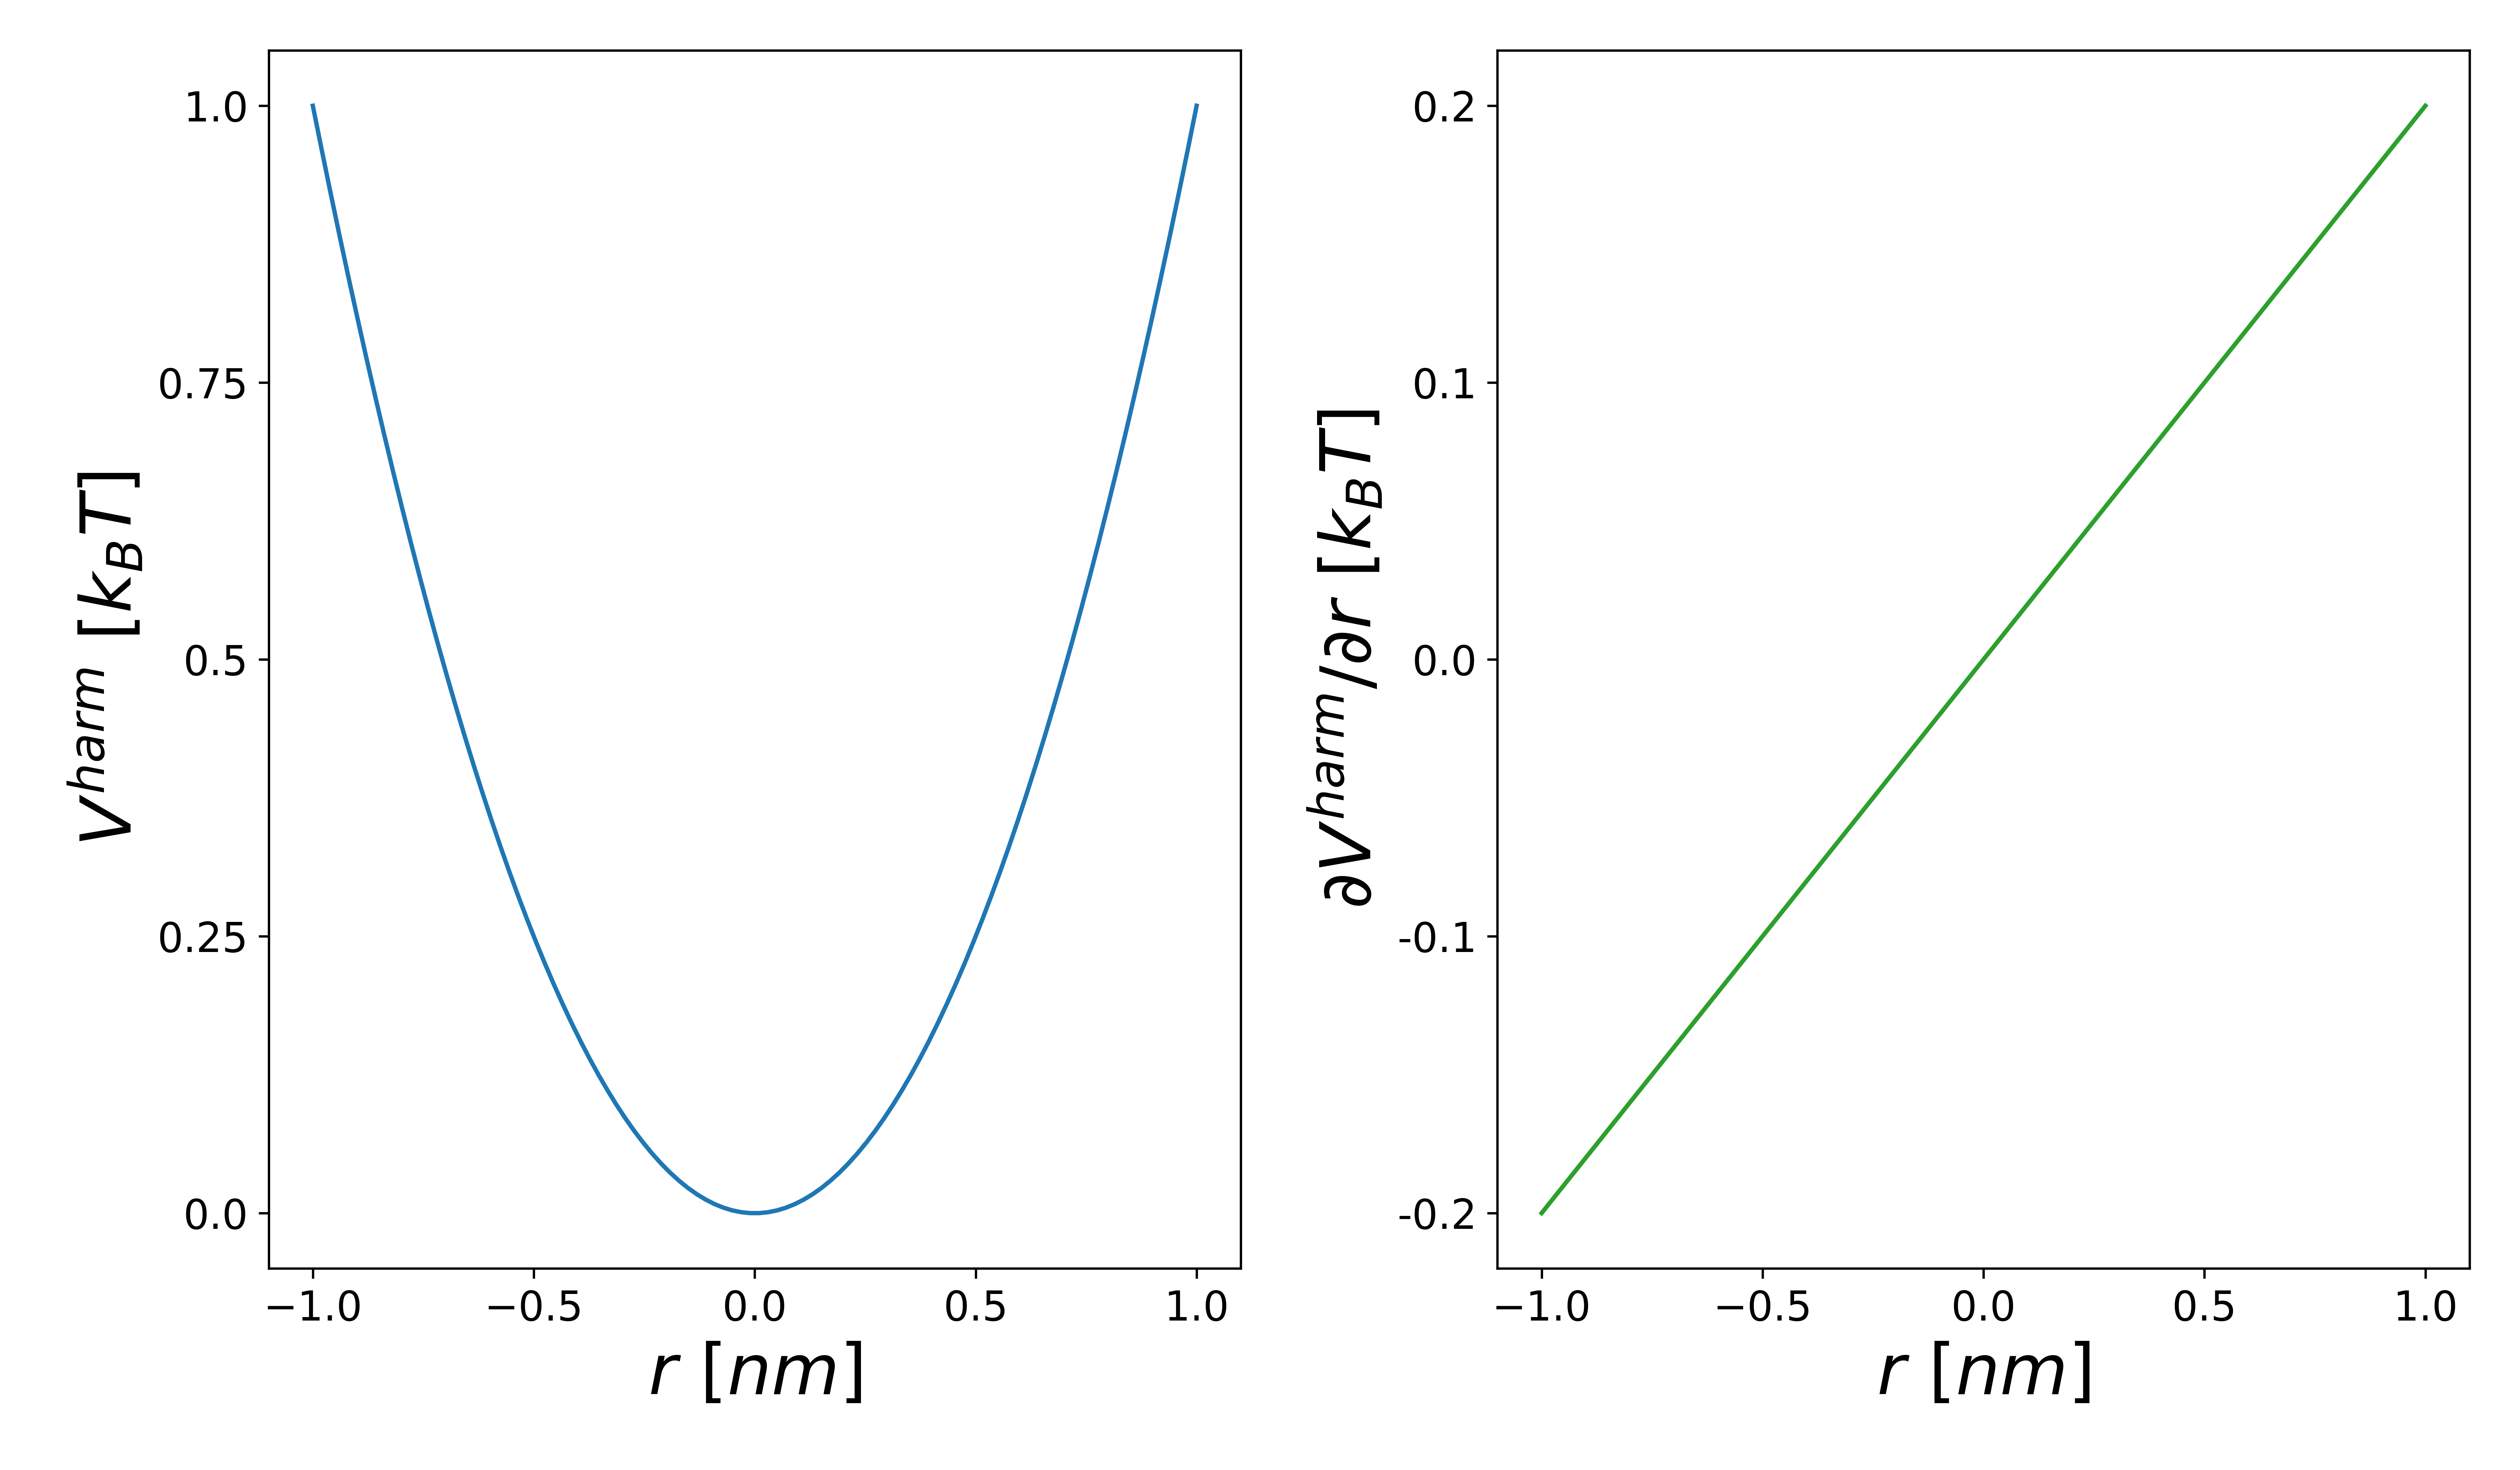
\includegraphics[width=\textwidth]{fig/ForceField/harm_osc.png}
    \caption{Harmonic Oscilator is a standard potential used for bond or angle bending in force fields}
    \label{fig:harmOsc}
\end{figure}

The GROMOS force field 54A7, however, uses a different form of the harmonic potential for computational reasons, \cite{Oostenbrink2004}
\begin{equation}
    V^{bond}(b_{ij}; K_{b_{ij}}, b^0_{ij})~=~\frac{1}{4} K^{quart}_{b_{ij}} (b_{ij}^2-{b_{ij}^{0}}^2)^2. \\
\end{equation}
The motivation of the special form of the bonded term  was reducing the number of square-root operations. \cite{}

In practice, the bond terms are replaced for large biomolecule simulations by Lagrange multiplier-based constraint algorithms such as the SHAKE\cite{Ryckaert1977, Ciccotti1986}, SETTLE\cite{Miyamoto1992} or the LINCS\cite{Hess1997} algorithm. \cite{} 
The usage of such constraint algorithms allows larger timesteps up to $2~fs$, increasing the efficiency of the MD simulation. \cite{}

\paragraph{Bond Angles}
The bonded terms describe the covalent bond-angle  interaction of three atoms. The angle of three atoms is derived as follow,
\begin{equation}
    \Theta_{ijk} = R_i, r_j, r_k
\end{equation}

In most force fields, this term is again used as a harmonic oscillator function. Nevertheless, GROMOS uses a different form of this definition,
\begin{equation}
    V^{angle}_{\theta_{ij}}~=~ \frac{1}{2} K_{\theta_{ijk}}(cos(\theta_{ijk})-cos(\theta^0_{ijk}))^2 \\
\end{equation}. \cite{Oostenbrink2004}
This form was chosen, in order to save an arcossine calculation for $\theta_{ijk}$ and is additionally  more robust. \cite{Oostenbrink2004}

\paragraph{Torsional Diherdal-Angle}
The torsion angle describes the rotation around a covalent bond. \cite{} It can be calculated from a set cooordinates of four atoms as,
\begin{equation}
    \delta_{o}(r_i, r_j, r_k, r_l) = sign(r_{ij} \cdot (r_{kj} \times r_{kl})) \arccos(\frac{(r_{i,j}\times r_{kj}) \cdot (r_{kj} \times r_{kl})}{(r_{i,j} \times r_{kj}) (r_{kj} \times r_{kl})}) \\
\label{eq:tangle}
\end{equation} 

The resulting potential function optimized for computation for GROMOS is,
\begin{equation}
    V^{torsion}(\phi_{ijkl}; K_{\phi_{ijkl}}, m_{ijkl}, \delta)~=~K_{\phi_{ijkl}}(1+cos(\delta)cos(m \phi_{ijkl})) \\
\end{equation}. \cite{Oostenbrink2004}
\begin{figure}[h]
    \centering
    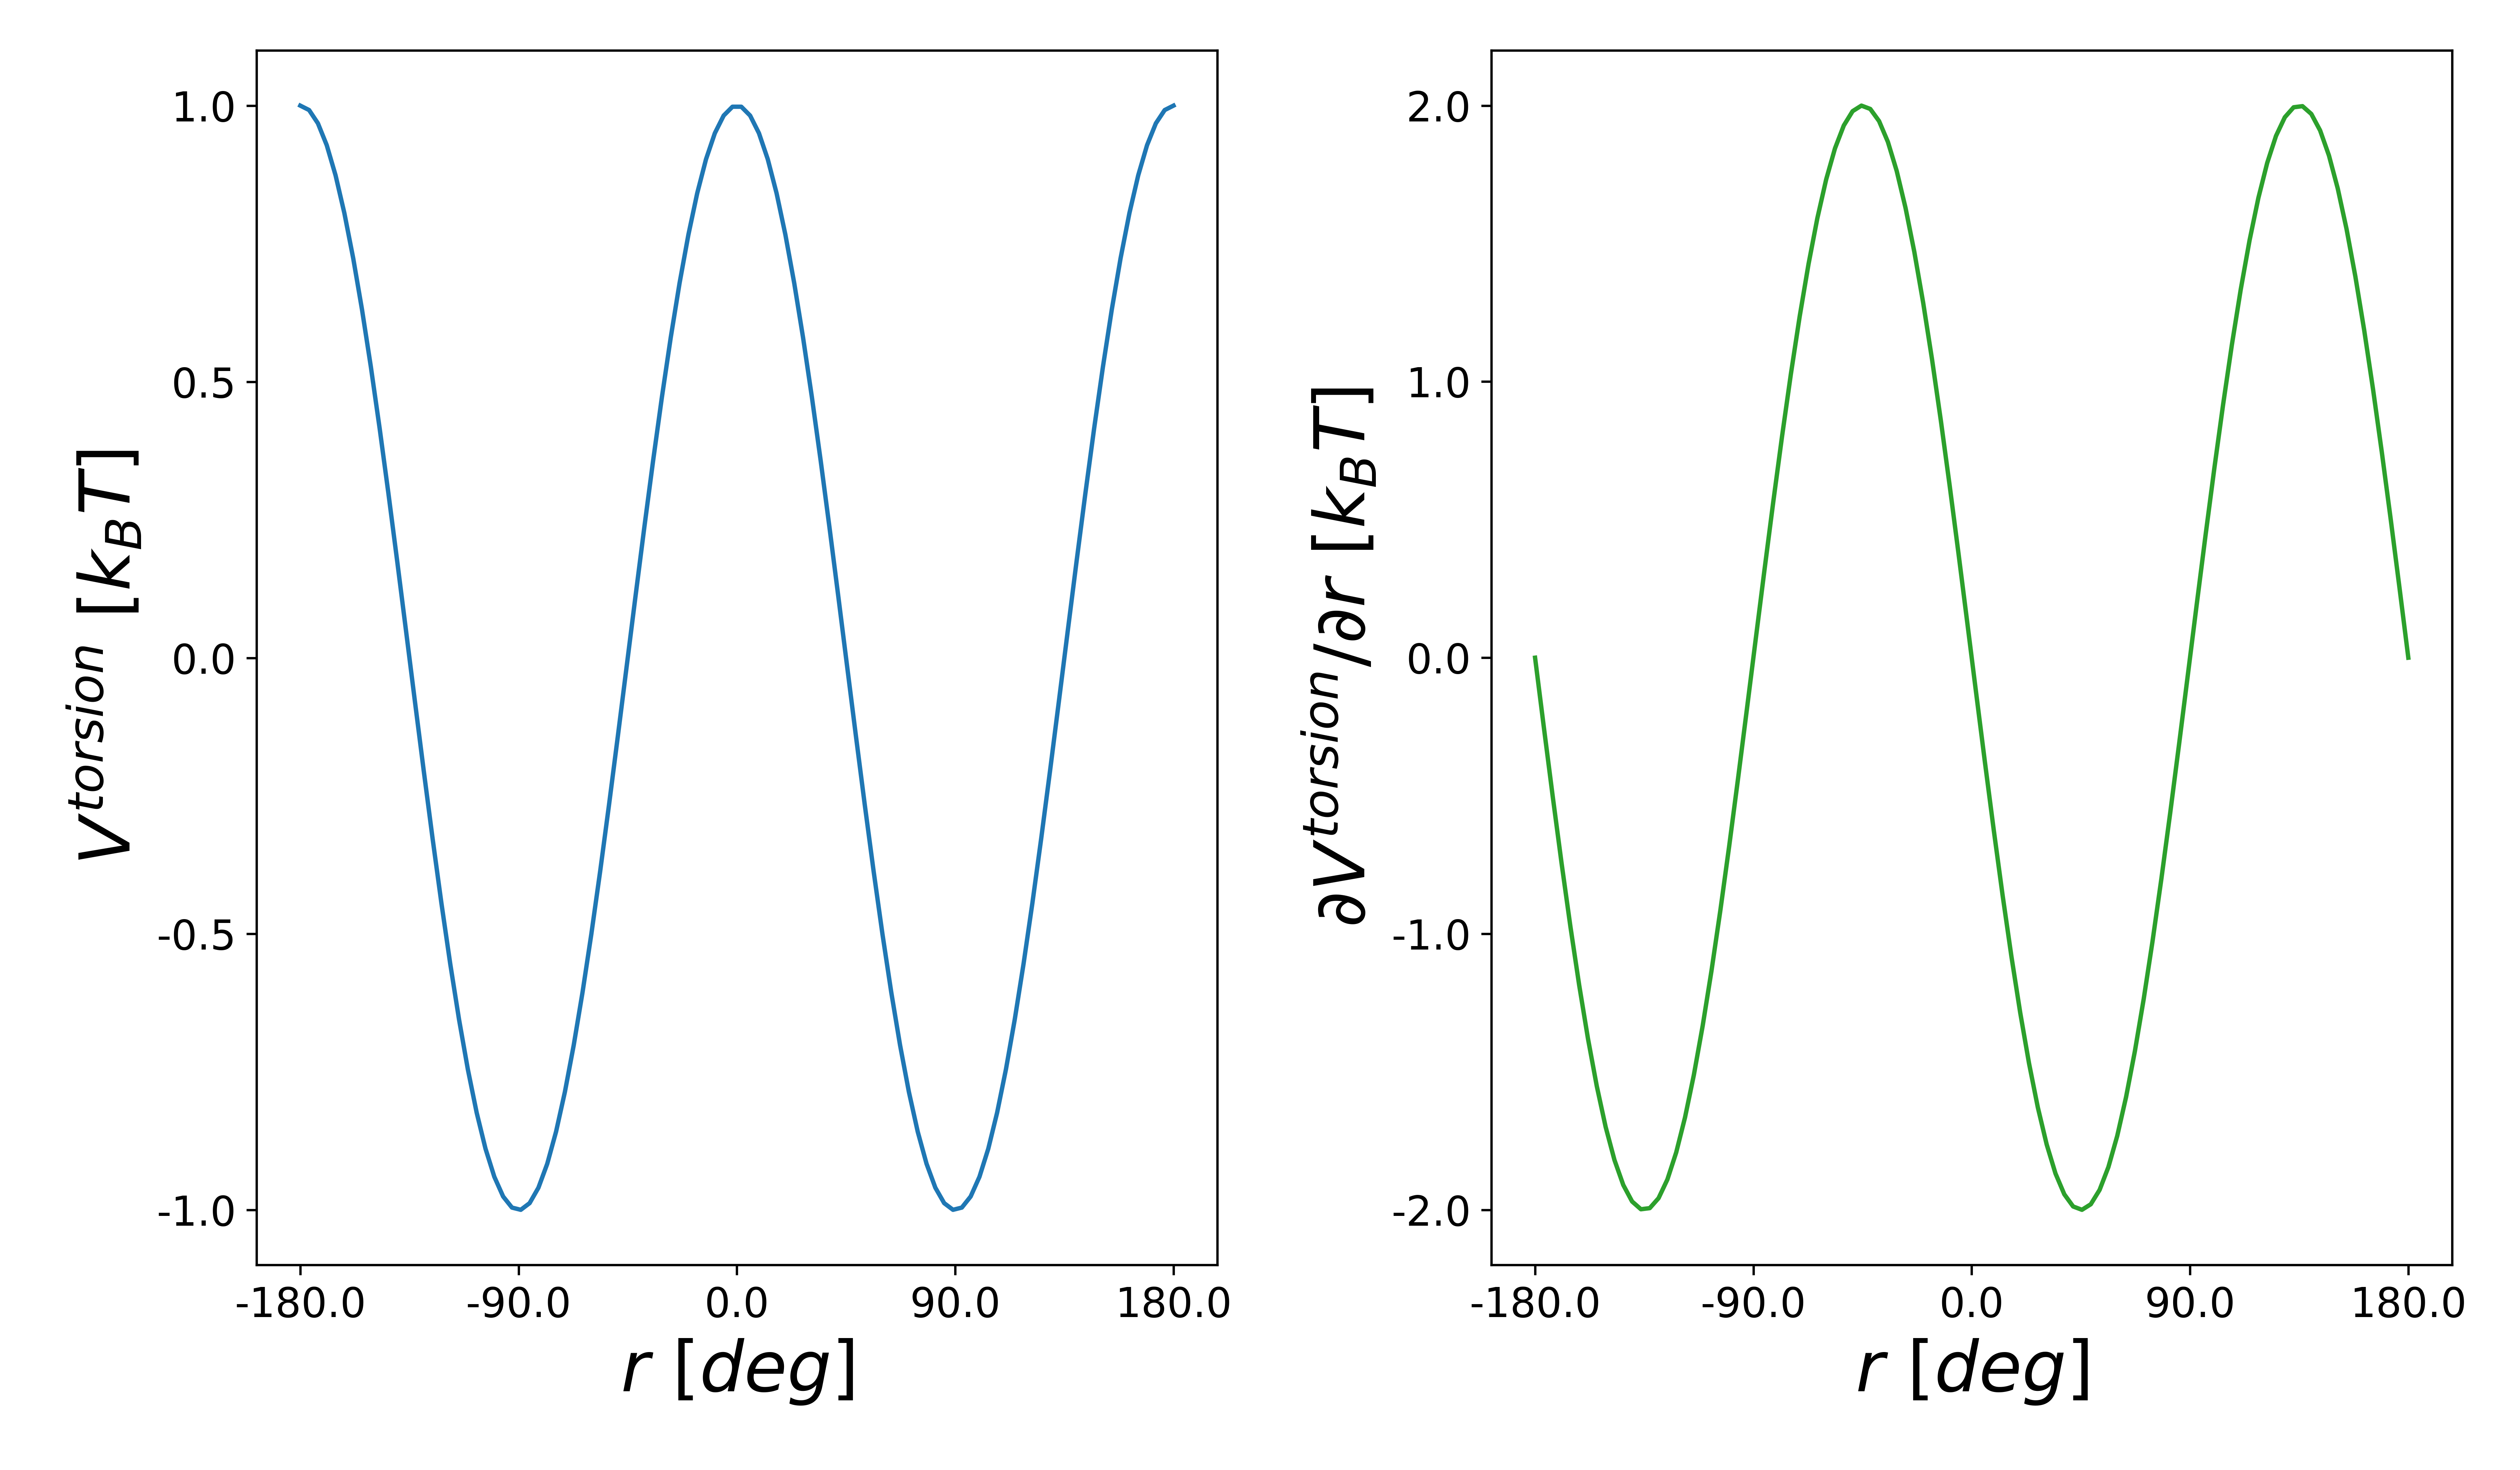
\includegraphics[width=\textwidth]{fig/ForceField/torsion.png}
    \caption{wave Potential is a standard potential used for bond or angle bending in force fields}
    \label{fig:torsion}
\end{figure}

\paragraph{Improper Diherdal-Angle}
Improper Dihedrals are used to properly build rotation barriers for molecules, like aromatic structures.\cite{Blondel1996}
\begin{equation}
    V^{improper}(\xi; k^{xi}_n) = k^{xi}_n (\xi_n - \xi^0_n)^2
\end{equation}
with $\xi$ as the out-of-plane distortion, it can be calculate like \ref{eq:tangle}. \cite{Oostenbrink2004}

\subsubsection{Nonbonded Terms}
The nonbonded interaction terms are split into two subterms: electrostatic and van der Waals interactions. These terms are the most computationally expensive ones as they need to be calculated for atom pairs depending on the distance to each other.

\paragraph{Electrostatic Interactions}
The interaction is modeled by a coulomb potential and describes the interactions of polar atoms.\cite{}
\begin{equation}
    V^{culomb}(r_i, r_j; q_i, q_j, \epsilon_0)  = \frac{q_i q_j}{4 \pi \sigma_0} \frac{1}{r_{ijW}}
\end{equation}. \cite{}

\begin{figure}[h]
    \centering
    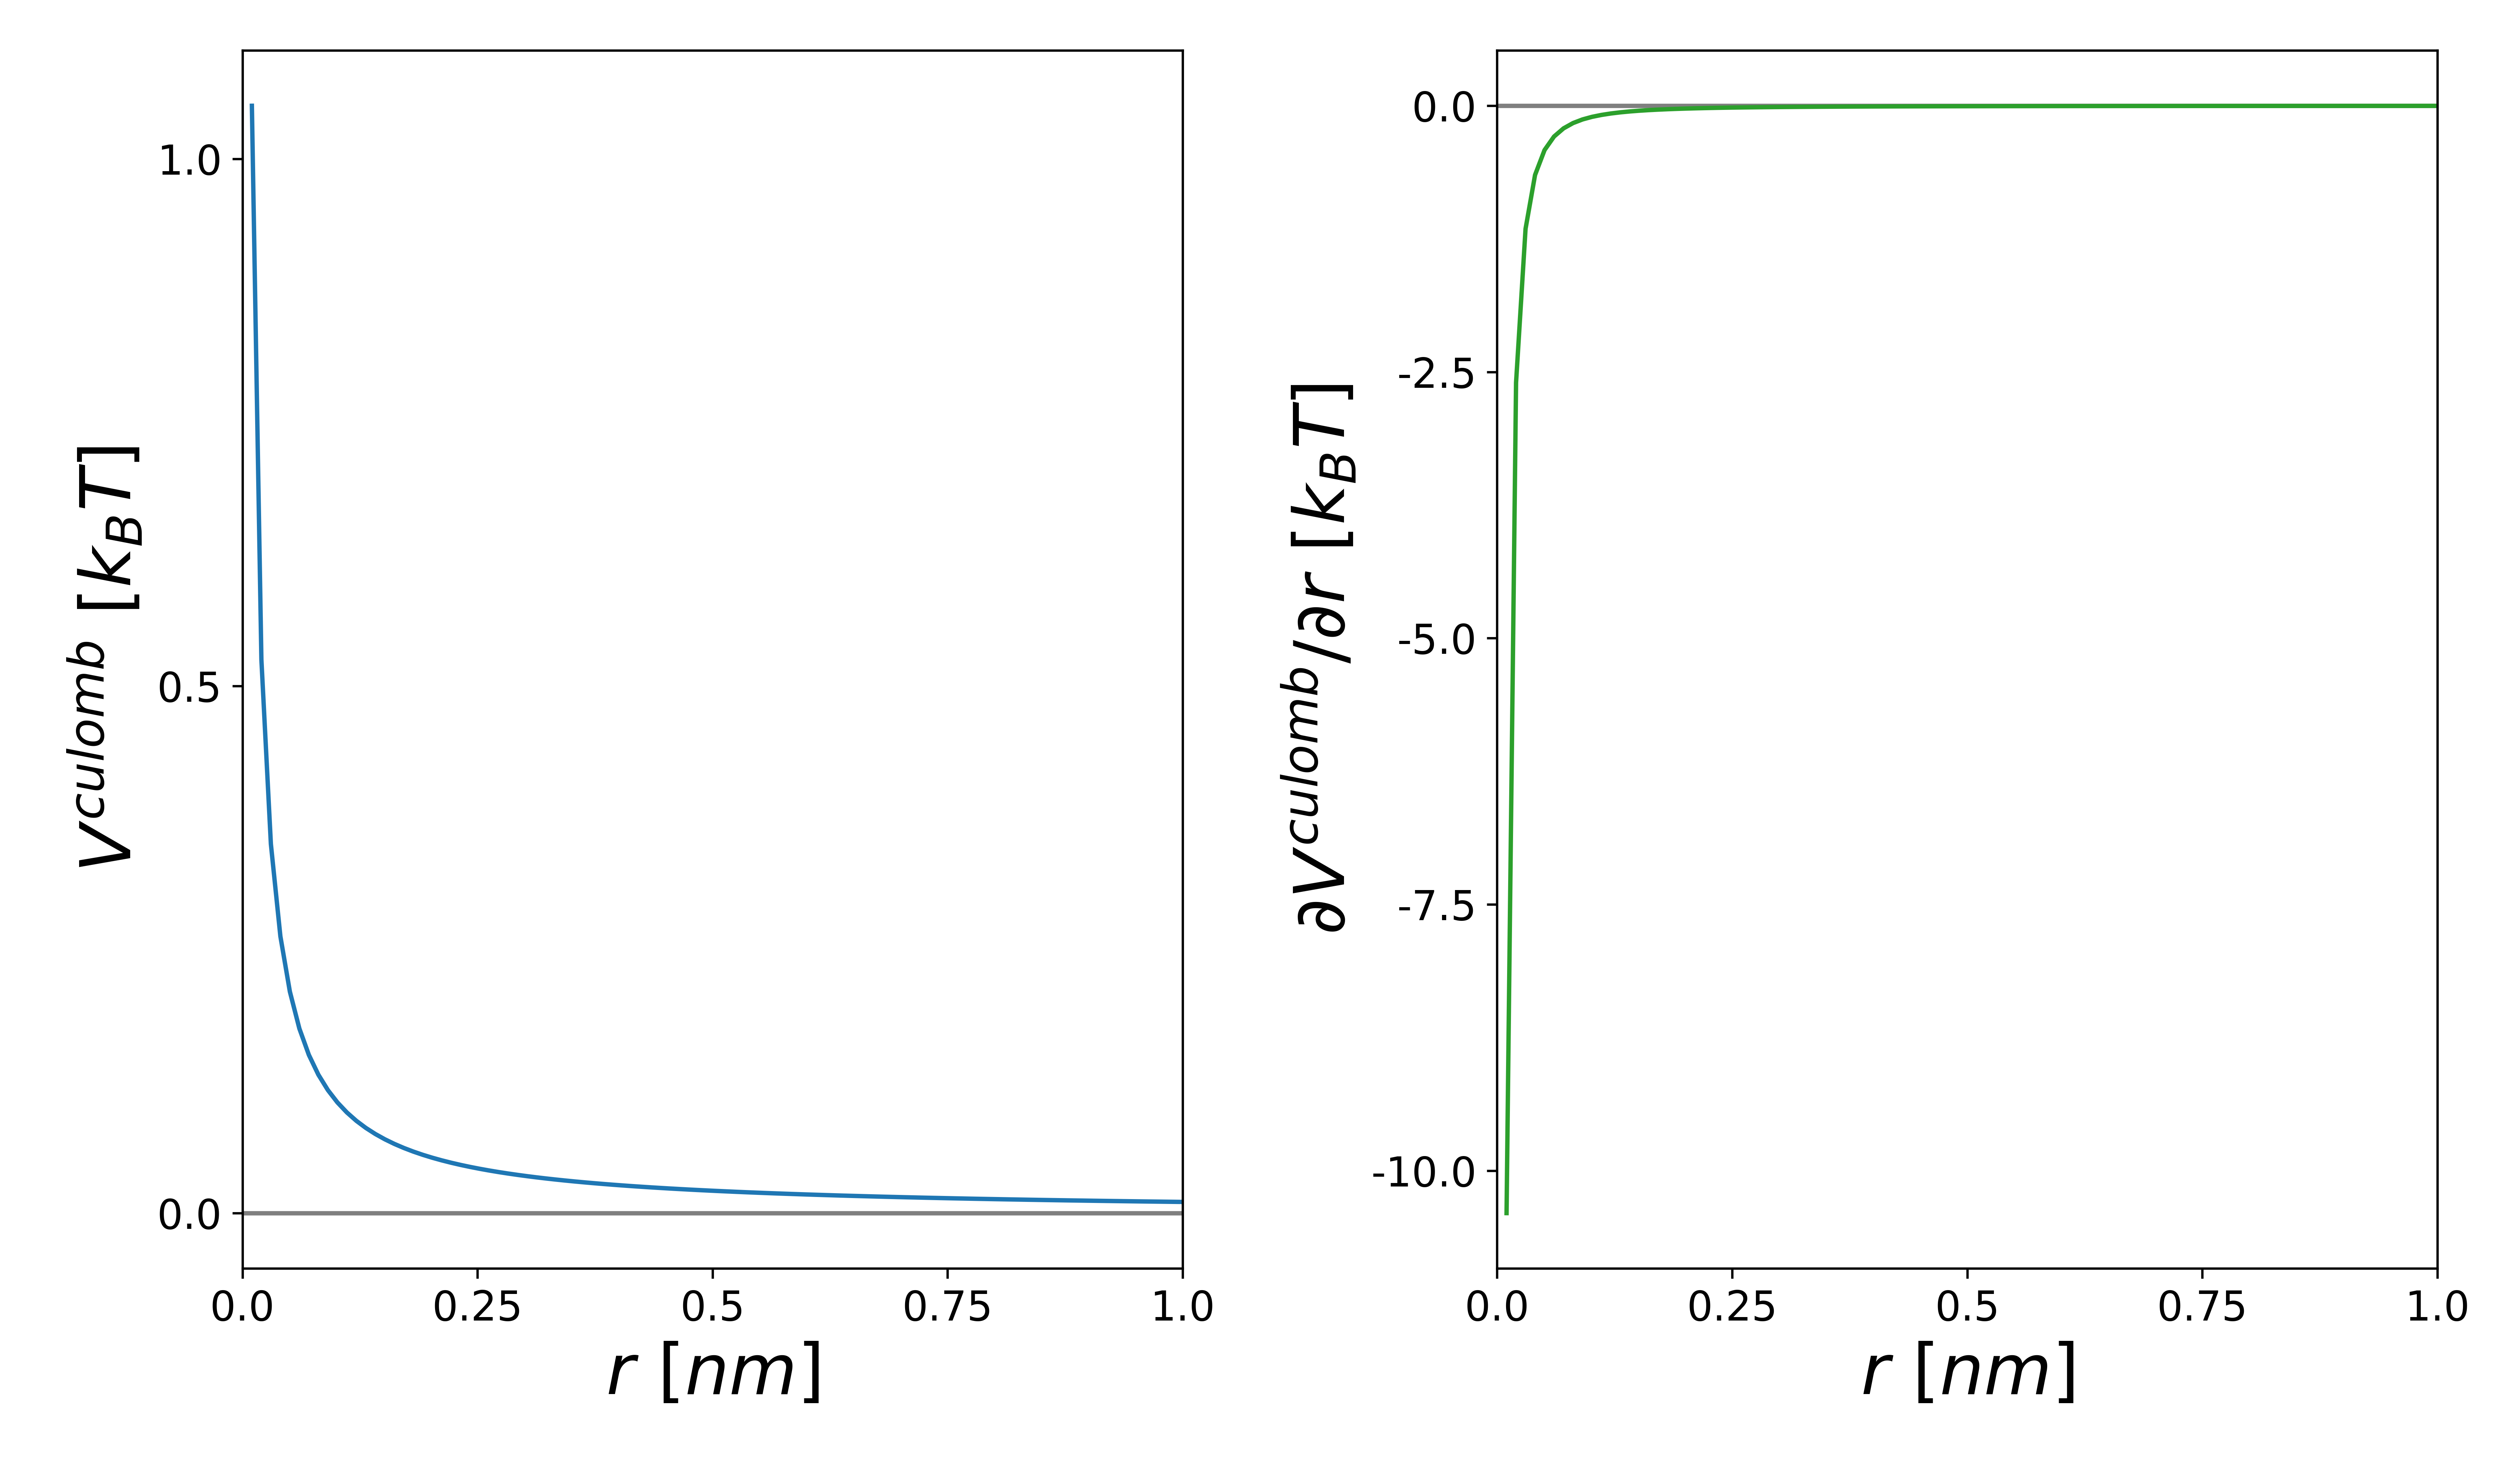
\includegraphics[width=\textwidth]{fig/ForceField/culomb.png}
    \caption{culomb is a standard potential used for bond or angle bending in force fields}
    \label{fig:culomb}
\end{figure}

In addition to this basic potential, Gromos adds two additional terms to add the reaction field contributions to the electrostatics, \cite{Tironi1995}

\paragraph{Van der Waals Interactions}
The Van der Waals term describes  ... and is often modeled with a Lennard-Jones 12/6 potential function \cite{Jones1924}.

GROMOS uses the  interaction function for describing these interactions. 
\begin{equation}
    V^{VdW}(r_{ij}; C6_{ij}, C12_{ij}) = (\frac{C12_{ij}}{r^{12}_ij}-\frac{C6_{ij}}{r^{6}_ij}) 
\end{equation}
with $r_{ij}$ the distance between two atoms, the parameters $C12_{ij}$ and $C6_{ij}$ depending on the atom types interacting with each other.
\begin{figure}[h]
    \centering
    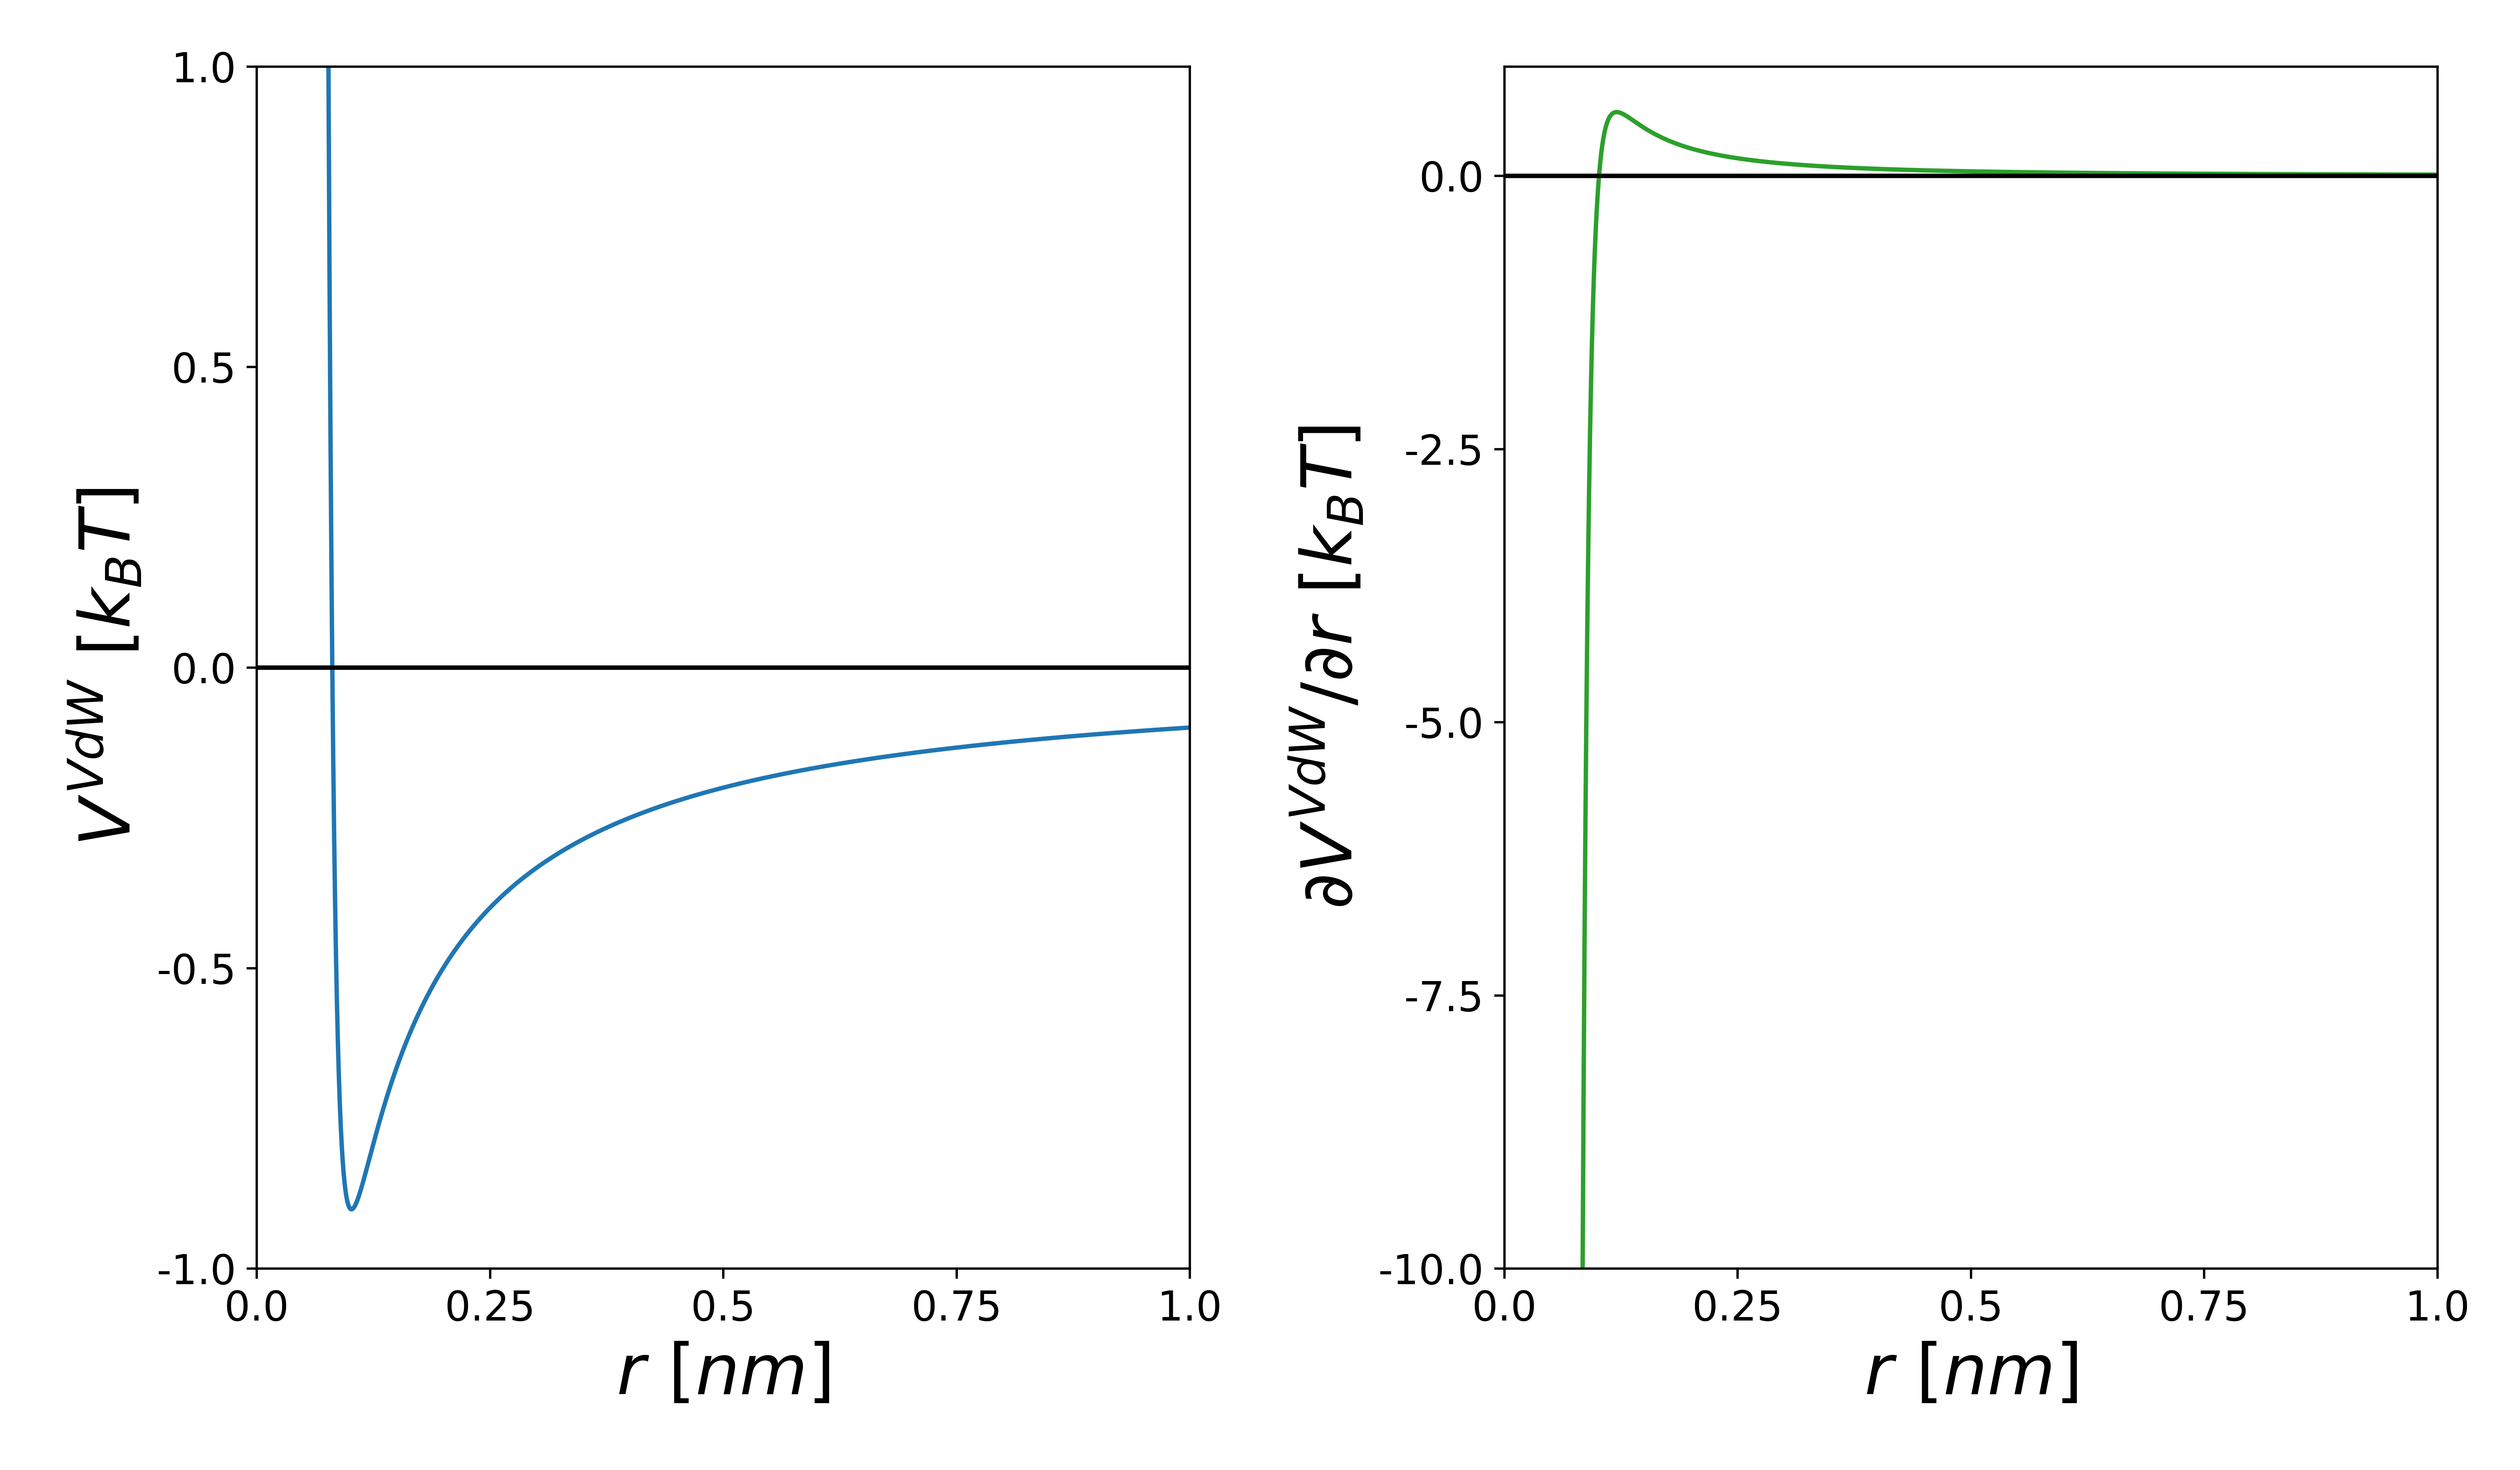
\includegraphics[width=\textwidth]{fig/ForceField/vdw.png}
    \caption{VdW Potential is a standard potential used for bond or angle bending in force fields}
    \label{fig:VdW}
\end{figure}



Multiple interaction functions are summed up to a force field function (FF). 
\begin{equation}
    V = V^{bonded} + V^{nonbonded} 
\end{equation}

The FF describes the total potential energy $V$ of a given coordinate set of a system $\textbf{r}$. The total coordinate space gives rise to the potential energy landscape (PES) defined by an FF.
During simulation, minima and barriers of the PES are explored and give insights into the conformational behavior of a system.

Many force fields functions and parameter sets were developed in the past, like for example: AMBER\cite{weiner1981,pearlman1995, cornell1995, LindorffLarsen2010}, GROMOS\cite{Daura1998, Oostenbrink2004, Schuler2001,Schmid2011, Malde2011, Stroet2018}, CHARMM\cite{brooks1983, mackerell1995,mackerell1998}, OPLS \cite{jorgensen1988, jorgensen1996} and OpenFF \cite{Qiu2021}
Additional molecules, that were not part of GROMOS54a7 were parametrised with the help of the Automated Topology Builder (ATB). \cite{Malde2011, Stroet2018}


% ------------------------ FREE ENERGY-------------------------------

%Probabilistic approach
The free energy difference $\Delta F$ between two states $A$ and $B$  can be calculated as,
\begin{equation}
    \begin{split}
        \Delta F_{AB} &= -\frac{1}{\beta} (\ln(p_A) - \ln(p_B)) 
                      &= -\frac{1}{\beta} \ln(\frac{p_A}{p_B})
    \end{split}
\end{equation}


The probabilities $p_A$ and $p_B$ can be calculated with different approaches, for example was the energy offset rebalancing in Chapter \ref{ch:fereeds} motivated by the direct counting methodology\cite{}. This approach uses sampled occurrences of a state x during a finite sampling approach to estimate the corresponding $p_x$. 

A different approach is used in relative alchemical free energy calculations due to the slow convergence of direct counting approaches for these problems \cite{}.
Here the Zwanzig equation \cite{Zwanzig1954} is employed using the Boltzmann weighted energy differences of the end-states to estimate $p_A$ and $p_B$.

\begin{equation}
    \begin{split}
        \Delta A_{AB} &= -\frac{1}{\beta} \ln \langle \frac{e^{- \beta V_A}}{e^{- \beta V_B}} \rangle_A
                      &= -\frac{1}{\beta} \ln \langle e^{- \beta (V_B-V_A)} \rangle_A
    \end{split}
\end{equation}

Many methods and approaches on how to calculate free energies from simulations were developed in the past. In Chapter 3 several will be discussed and in Chapter 2-3 we will expand the methodology of RE-EDS and the linked dual topology approach.

If the used ensemble was a canonical ensemble, the resulting free energy is a Helmholtz free energy, under the isothermal-isobaric condition a Gibbs free energy is retrieved.

This equation only leads to good results, if the phase space overlap of the end states is large enough. \cite{}
Multiple possible solutions were found to bridge the phase space, like the linear state coupling used in thermodynamic integration (TI) \cite{Kirkwood1935}, the exponential state coupling used in enveloping distribution sampling (EDS) \cite{Christ2007}, or the hybrid method $\lambda$-EDS \cite{Koenig2020} combining both approaches. In Chapter \ref{ch:feens} different methodologies and their sampling behavior will be illustrated with toy model in the application example of and in Chapter \ref{ch:fereeds} a detailed example of automatizing and studying the sampling behavior of replica-exchange - EDS (RE-EDS)\cite{Sidler2016} is provided.
A last, but fundamental aspect of relative alchemical free energy calculations is how the two end-states are represented in a system. To this problem multiple solutions were proposed in the past. A Categorization of the different approaches and further development of one aspect of the methodology is introduced in Chapter \ref{ch